\documentclass[a4j,10pt,dvipdfmx]{jarticle}
\usepackage{siunitx}
\usepackage[dvipdfmx]{graphicx}
\usepackage{pdfpages}
\usepackage{here}
\usepackage{listings,jlisting}
\usepackage{tabularx}
\lstset{
  basicstyle={\ttfamily},
  identifierstyle={\small},
  commentstyle={\smallitshape},
  keywordstyle={\small\bfseries},
  ndkeywordstyle={\small},
  stringstyle={\small\ttfamily},
  frame={tb},
  breaklines=true,
  columns=[l]{fullflexible},
  numbers=left,
  xrightmargin=0zw,
  xleftmargin=3zw,
  numberstyle={\scriptsize},
  stepnumber=1,
  numbersep=1zw,
  lineskip=-0.5ex
}
\begin{document}
\title{微分方程式の課題}
\author{学籍番号2120029, 氏名 政野玄空}
\date{2023年8月16日}
\maketitle
\section{レポート課題1}

まず$\frac{dy}{dt} = f(t,y)$,初期値が$y_0$ = 1.0, $t_0$ = 0.0, $dt$ = 0.1のオイラー法のコードを提示する.
\begin{lstlisting}[label=prm1, caption=kadai5-1]
  #include <stdio.h>
  #include <math.h>
  
  int main(void) {
      double y = 1.0;
      double t = 0.0;
  
      double dt = 0.1;
      while (t < 10.0) {
          t += dt;
          y += dt * y;
          printf("%f,%f \n",t,y);
      }
      return 0;
  }  
\end{lstlisting}
今回は39行目のdtと42行目のtを変化させて実行し,$\Delta$y表を作成する.$\Delta$yは$\left| \frac{数値解-厳密解}{数値解} \right|$で計算する.
\begin{table}[H]
  \label{1}
  \begin{center}
  \caption{表1}
  \begin{tabular}{|l|l|l|l|l|l|}
  \hline
      手法 & \multicolumn{5}{|c|}{計算終了時間} \\\cline{2-6}
      & 2 & 4 & 6 & 8 & 10 \\ \hline
      オイラー法:dt = 0.1 & 8.953187e-02 & 1.710478e-01 & 2.452654e-01 & 3.128382e-01 & 3.743611e-01 \\ \hline
      オイラー法:dt = 0.025 & 2.429106e-02 & 4.799214e-02 & 7.111745e-02 & 9.368103e-02 & 1.156965e-01 \\ \hline
  \end{tabular}
\end{center}
\end{table}
dtの値が小さくなればなるほどyの相対誤差が小さくなることが確認できた.

\section{レポート課題2-1}
まず$\frac{dy}{dt} = f(t,y)$,初期値が$y_0$ = 1.0, $t_0$ = 0.0, $dt$ = 0.2の4次のルンゲクッタ法のコードを提示する.
オイラー法については同様のコードのk1の値をyに足す,2次のルンゲクッタ法については同様のコードのk2の値をyに足すことで計算できるので省略する.
\begin{lstlisting}[label=prm3, caption=4次のルンゲクッタ法]
  #include <stdio.h>
  #include <math.h>
  
  double f(double y) {
     return y; 
  }
  // 4nd Runge-Kutta Method
  void rungeKutta(double t0, double y0, double dt, double t_end) {
      double t = t0;
      double y = y0;
  
      while (t < t_end) {
          double k1 = dt*f(y);
          double k2 = dt*f(y + (k1 / 2.0));
          double k3 = dt*f(y + (k2 / 2.0));
          double k4 = dt*f(y + k3);
          double exacty = exp(t);
          printf("Runge-Kutta Method\n");
          printf("t = %f, y = %f\n", t, y);
          printf("Exact Solution\n");
          printf("t = %f, y = %f\n", t, exacty);
          printf("relative error\n");
          printf("t = %f, deltay = %e\n", t, fabs((y-exacty)/exacty));
          y += (k1+2*k2+2*k3+k4)/6;
          t += dt;
      }
  }
  
  int main() {
      double t0 = 0.0;
      double y0 = 1.0;
      double dt = 0.2;
      double t_end = 10.0;
  
      printf("Runge-Kutta Method\n");
      rungeKutta(t0, y0, dt, t_end);
  
      return 0;
  }
  
\end{lstlisting}
それぞれdtの値を0.2,0.1,0.05,0.025,0.0125に変更してレポート課題2-1の表を完成させる.
\begin{table}[H]
  \label{2}
  \begin{center}
  \caption{表2}
  \begin{tabular}{|l|l|l|l|l|l|}
  \hline
      手法 & \multicolumn{5}{|c|}{タイムステップ $\Delta$t} \\\cline{2-6}
      & 0.2 & 0.1 & 0.05 & 0.025 & 0.0125 \\ \hline
      オイラー法 & 5.868407e-01 & 3.743612e-01 & 2.139677e-01 & 1.154246e-01 & 6.010208e-02 \\ \hline
      2次ルンゲクッタ法 & 5.583757e-02 & 1.534751e-02 & 3.985508e-03 & 1.019255e-03 & 2.579542e-04 \\ \hline
      4次ルンゲクッタ法 & 1.129033e-04 & 7.667773e-06 & 4.970922e-07 & 3.180150e-08 & 2.013389e-09 \\ \hline
  \end{tabular}
\end{center}
\end{table}
\section{レポート課題2-2}
エクセルで同様の表を作成し,グラフを作成した.
\begin{figure}[H]
  \begin{center}
  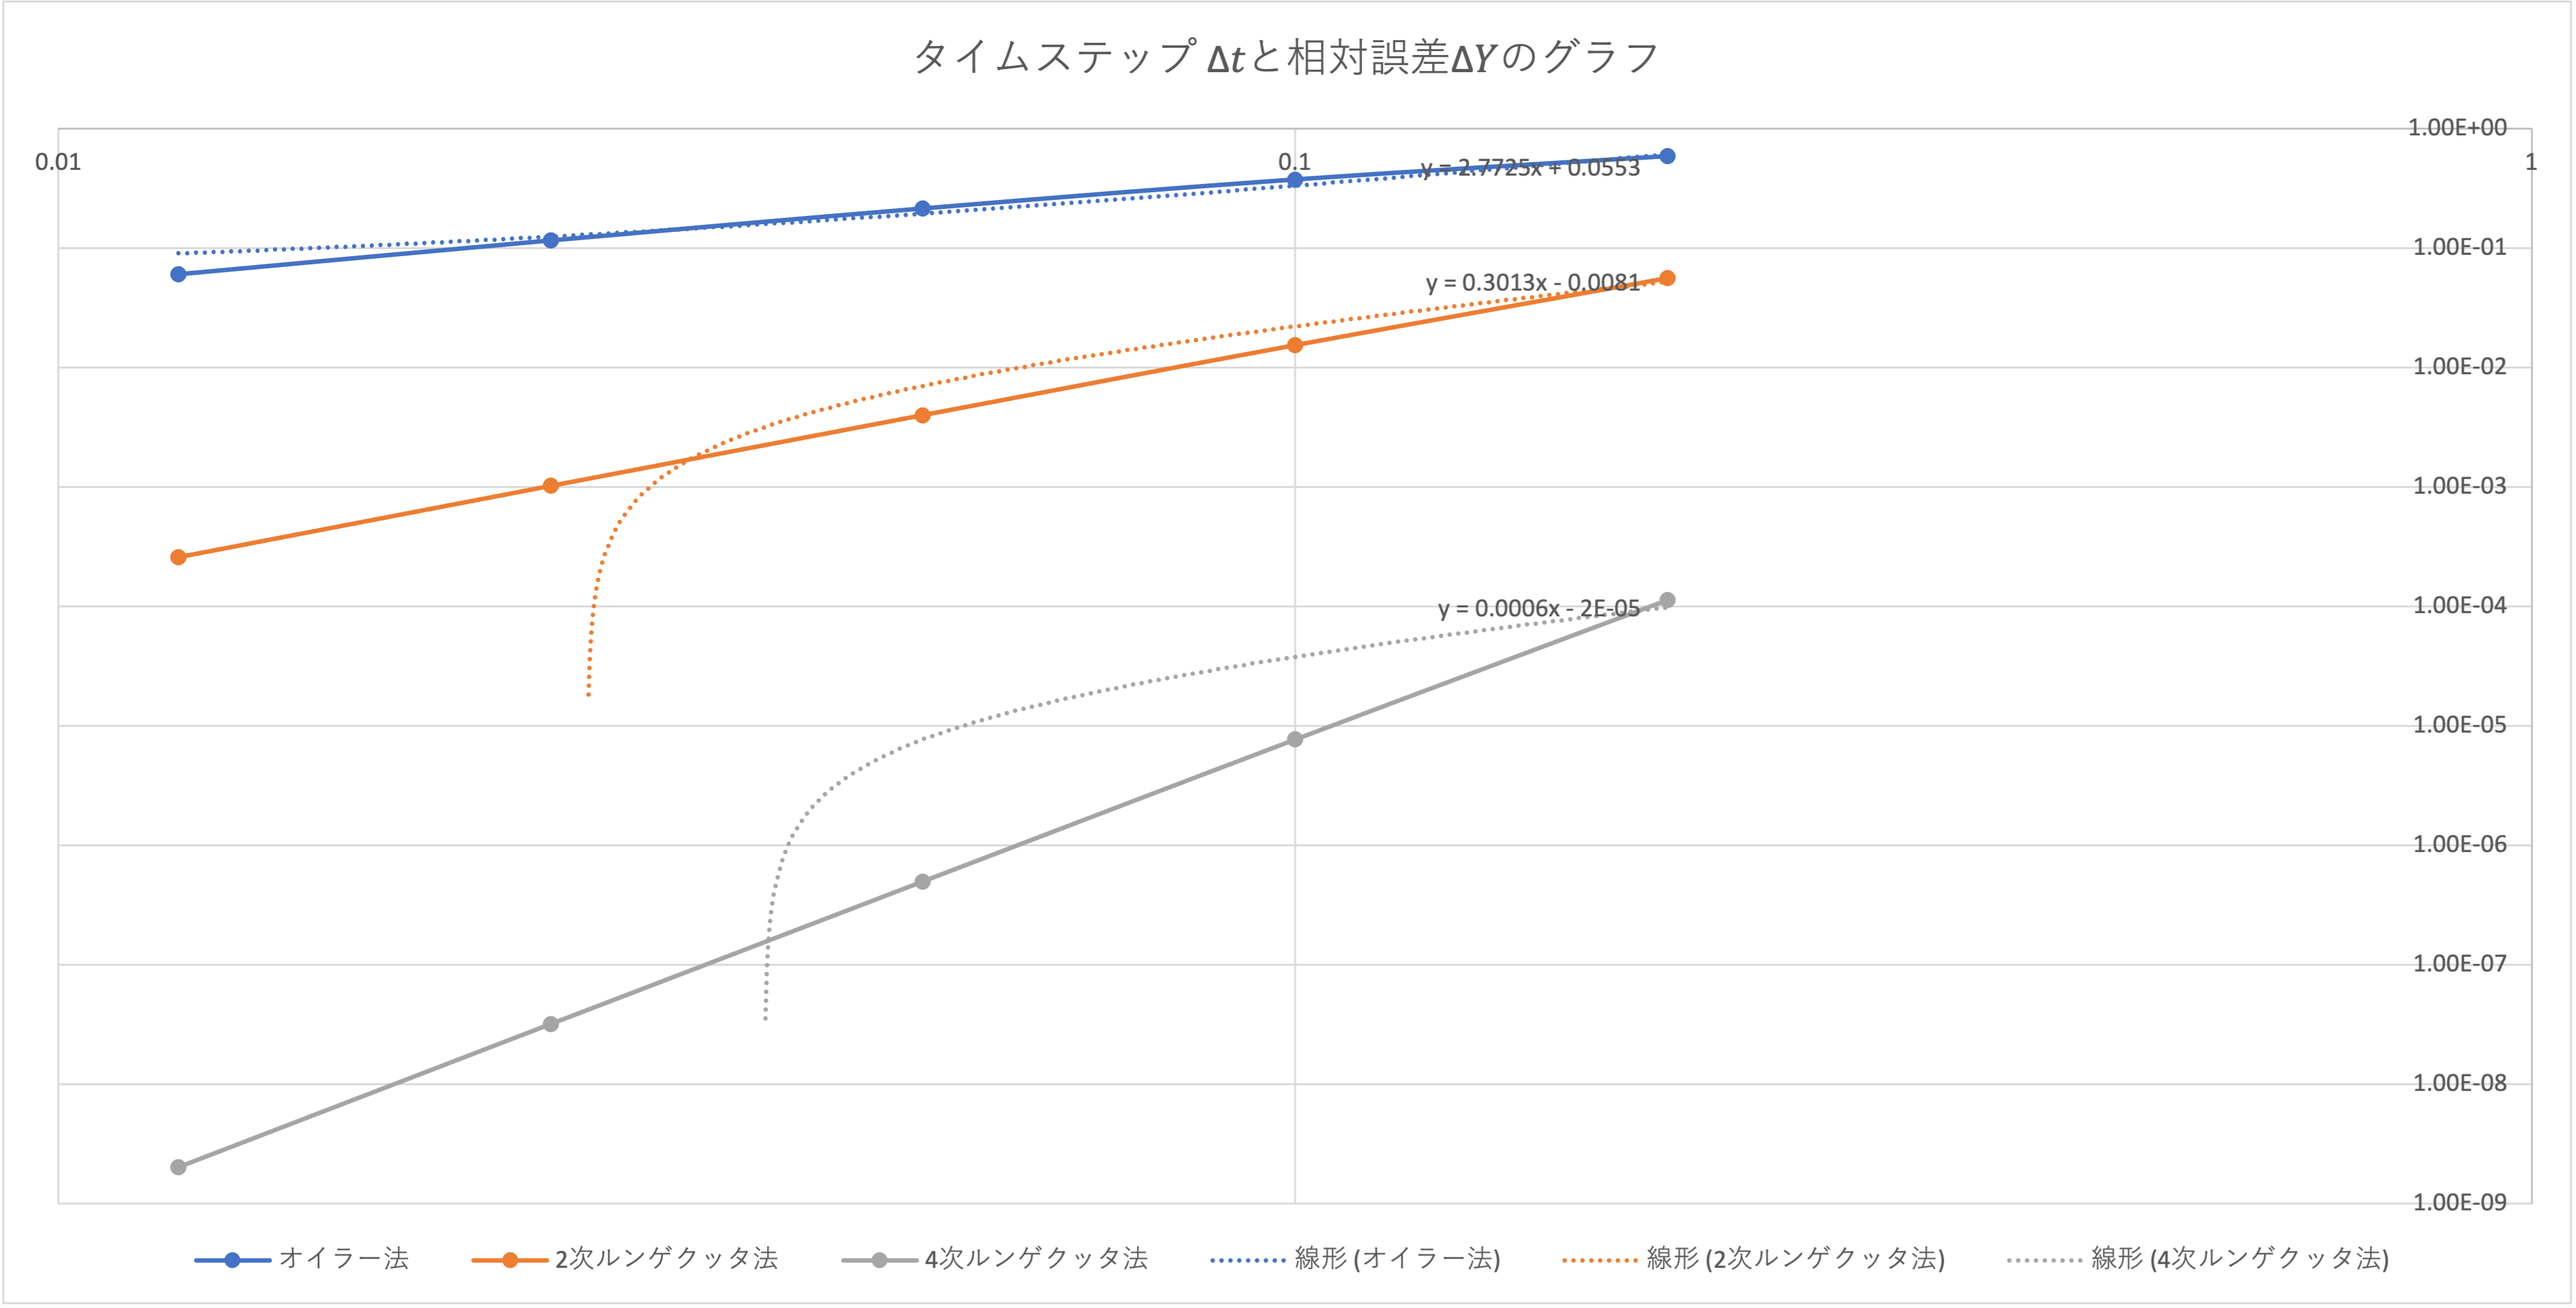
\includegraphics[height=7cm,width=10cm]{2-2.png}
  \caption{タイムステップ$\Delta$tと相対誤差$\Delta$Yのグラフ}
\end{center}
\end{figure}
傾きはオイラー法が2.7723,2次のルンゲクッタ法が0.3013,4次のルンゲクッタ法が0.0006となった.
\section{レポート課題2-3}
各方法のタイムステップを小さくする利点と欠点を考察していく.
\subsection{オイラー法}
利点:精度が向上し近似的な解が真の解により近づく.
欠点:tの範囲が小さくても高い精度を得るためには多くのステップが必要になり計算量が大きくなる.
\subsection{2次のルンゲクッタ法}
利点:タイムステップを短くすることで,数値解の精度が向上し,オイラー法よりも高い精度の結果を得ることができるうえにオイラー法に比べて収束性が向上し,安定して解を得ることができる.
欠点:タイムステップを短くすると,計算量が増加する.しかし,4次ランゲクッタ法に比べては計算量は少ない.
\subsection{4次のルンゲクッタ法}
利点:高い数値解の精度を持つ.近似的な解を高次の精度で求めることができる.タイムステップを短くしても,高次の精度を保ちながら計算を行える.
欠点:計算量が多くなる.タイムステップを非常に小さくする場合,高い精度を保つことができるが,計算コストが増加する.

それぞれタイムステップを小さくする場合は精度が向上するが,計算量が増加し,特に4次のルンゲクッタ法は顕著である.またタイムステップを小さくしすぎると数値誤差が累積していき問題になる場合もある.
問題によって計算時間とリソースを考慮し適切な方法を選ぶのが重要だと考えられる.
\end{document}
